\mysection{Prblem Set 1.2}

\begin{description}
  \setlength{\parskip}{0cm} % 段落間
  \setlength{\itemsep}{0cm} % 項目間
  \item[8 (a) 回答] Tomは、3 回握手をした。
  \item[8 (b) 回答] Tomの妻は、3 回握手をした。
\end{description}

問題の解を与えるグラフを下図に示す。
Coupleは、夫婦の内、夫、妻のどちらかを表す。
\\


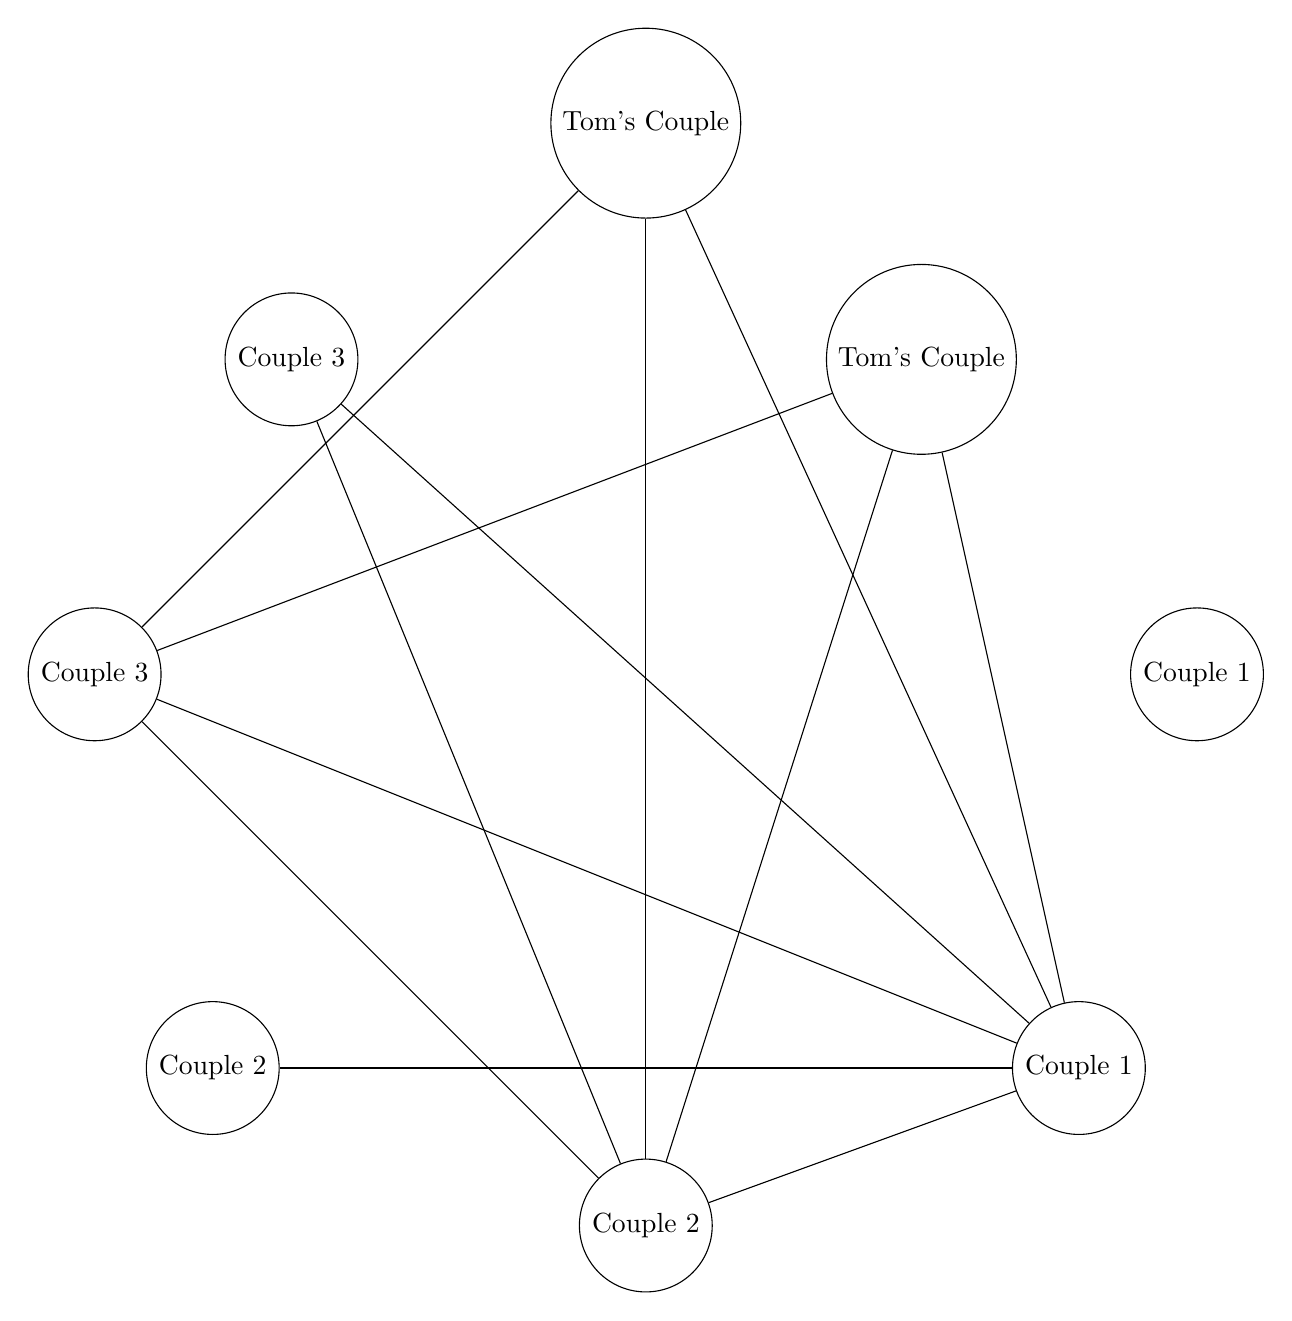
\begin{tikzpicture}[every node/.style={circle,draw}]
  \node (A) at (12.5, 2) {Couple 1};
  \node (B) at (7, 0) {Couple 2};
  \node (C) at (1.5, 2) {Couple 2};
  \node (D) at (0, 7) {Couple 3};
  \node (E) at (2.5, 11) {Couple 3};
  \node (F) at (7, 14) {Tom's Couple};
  \node (G) at (10.5, 11) {Tom's Couple};
  \node (H) at (14, 7) {Couple 1};
  \foreach \u \v in {A/B, A/C, A/D, A/E, A/F, A/G, B/D, B/E, B/F, B/G, D/F, D/G}
      \draw (\u) -- (\v);
\end{tikzpicture}

\mysection{Problem Set 1.8}

\begin{description}
  \setlength{\parskip}{0cm} % 段落間
  \setlength{\itemsep}{0cm} % 項目間
  \item[8 回答] $p=p_1\cdot p_2$, $q=p_1\cdot q_2+p_2 \cdot q_1$
\end{description}